\subsubsection{Manually pull up \texttt{TX\_DATAVALID}}
DCB pilot boards do not have pull-up resistor to pull up \texttt{TX\_DATAVALID}
automatically.
This would prevent PRBS tests, since without it pulling up, MiniDAQ would
consider data frames as ``invalid''\footnote{
    Which is not really the case, as all \texttt{TX\_DATAVALID} does is flip
    single bit 0 to 1 on the header part of the data frame.
}.

A large ($\approx$ 5~k$\Omega$) resistor is connected between the \emph{data
GBTx} FFC breakout board \texttt{TX\_DATAVALID} pin and 1.5~V rail.
See \autoref{fig:dcb_tx_datavalid_pull_up} for connection details.

\begin{figure}[!ht]
\centering
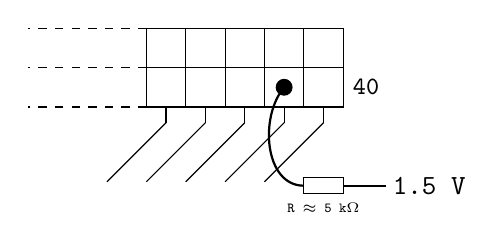
\begin{tikzpicture}
    % Pins
    \draw (0,0) rectangle (0.5,0.5);
    \draw (0.5,0) rectangle (1,0.5);
    \draw (1,0) rectangle (1.5,0.5);
    \draw (1.5,0) rectangle (2,0.5);
    \draw (2,0) rectangle (2.5,0.5);

    \draw (0,-0.5) rectangle (0.5,0);
    \draw (0.5,-0.5) rectangle (1,0);
    \draw (1,-0.5) rectangle (1.5,0);
    \draw (1.5,-0.5) rectangle (2,0);
    \draw (2,-0.5) rectangle (2.5,0);

    % Extension lines
    \draw [dashed] (0,0.5) -- (-1.5,0.5);
    \draw [dashed] (0,0) -- (-1.5,0);
    \draw [dashed] (0,-0.5) -- (-1.5,-0.5);

    % Additional copper traces
    \draw (0.25,-0.5) -- (0.25,-0.7);
    \draw (0.75,-0.5) -- (0.75,-0.7);
    \draw (1.25,-0.5) -- (1.25,-0.7);
    \draw (1.75,-0.5) -- (1.75,-0.7);
    \draw (2.25,-0.5) -- (2.25,-0.7);

    \draw (0.25,-0.7) -- (-0.5,-1.45);
    \draw (0.75,-0.7) -- (0,-1.45);
    \draw (1.25,-0.7) -- (0.5,-1.45);
    \draw (1.75,-0.7) -- (1,-1.45);
    \draw (2.25,-0.7) -- (1.5,-1.45);

    % Helper labels (imaginary)
    \coordinate (B) at (2.5,-0.25);
    \node at (B) [right] {\small\texttt{40}};

    % TX_DATAVALID pin
    \draw [black,fill] (1.75,-0.25) circle [radius=0.1];
    \draw [black,thick] (1.75,-0.25) to [out=-130,in=180] (2,-1.5) node {};
    \draw (2,-1.4) rectangle (2.5,-1.6);
    \draw [black,thick] (2.5,-1.5) to [out=0,in=0] (3,-1.5)
        node [right] {\texttt{1.5~V}};

    % Resistor label
    \coordinate (A) at (2.25,-1.6);
    \node at (A) [below] {\tiny\texttt{R $\approx$ 5~k$\Omega$}};
\end{tikzpicture}
\caption{
    Manually pull up \texttt{TX\_DATAVALID} with a large resistor connected to
    1.5~V rail.
    Pay attention to the orientation of the FFC breakout board.
}
\label{fig:dcb_tx_datavalid_pull_up}
\end{figure}
